\documentclass[
  bibliography=totoc,     % Literatur im Inhaltsverzeichnis
  captions=tableheading,  % Tabellenüberschriften
  titlepage=firstiscover, % Titelseite ist Deckblatt
]{scrartcl}

% Paket float verbessern
\usepackage{scrhack}

% Warnung, falls nochmal kompiliert werden muss
\usepackage[aux]{rerunfilecheck}

% unverzichtbare Mathe-Befehle
\usepackage{amsmath}
% viele Mathe-Symbole
\usepackage{amssymb}
% Erweiterungen für amsmath
\usepackage{mathtools}

% Fonteinstellungen
\usepackage{fontspec}
% Latin Modern Fonts werden automatisch geladen
% Alternativ:
%\setromanfont{Libertinus Serif}
%\setsansfont{Libertinus Sans}
%\setmonofont{Libertinus Mono}
\recalctypearea % Wenn man andere Schriftarten gesetzt hat,
% sollte man das Seiten-Layout neu berechnen lassen

% deutsche Spracheinstellungen
\usepackage{polyglossia}
\setmainlanguage{german}


\usepackage[
  math-style=ISO,    % ┐
  bold-style=ISO,    % │
  sans-style=italic, % │ ISO-Standard folgen
  nabla=upright,     % │
  partial=upright,   % ┘
  warnings-off={           % ┐
    mathtools-colon,       % │ unnötige Warnungen ausschalten
    mathtools-overbracket, % │
},                       % ┘
]{unicode-math}

% traditionelle Fonts für Mathematik
\setmathfont{Latin Modern Math}
% Alternativ:
%\setmathfont{Libertinus Math}

\setmathfont{XITS Math}[range={scr, bfscr}]
\setmathfont{XITS Math}[range={cal, bfcal}, StylisticSet=1]

% Zahlen und Einheiten
\usepackage[
locale=DE,                   % deutsche Einstellungen
separate-uncertainty=true,   % immer Fehler mit \pm
per-mode=symbol-or-fraction, % / in inline math, fraction in display math
]{siunitx}

% chemische Formeln
\usepackage[
version=4,
math-greek=default, % ┐ mit unicode-math zusammenarbeiten
text-greek=default, % ┘
]{mhchem}

% richtige Anführungszeichen
\usepackage[autostyle]{csquotes}

% schöne Brüche im Text
\usepackage{xfrac}

% Standardplatzierung für Floats einstellen
\usepackage{float}
\floatplacement{figure}{htbp}
\floatplacement{table}{htbp}

% Floats innerhalb einer Section halten
\usepackage[
section, % Floats innerhalb der Section halten
below,   % unterhalb der Section aber auf der selben Seite ist ok
]{placeins}

% Seite drehen für breite Tabellen: landscape Umgebung
\usepackage{pdflscape}

% Captions schöner machen.
\usepackage[
  labelfont=bf,        % Tabelle x: Abbildung y: ist jetzt fett
  font=small,          % Schrift etwas kleiner als Dokument
  width=0.9\textwidth, % maximale Breite einer Caption schmaler
]{caption}
% subfigure, subtable, subref
\usepackage{subcaption}

% Grafiken können eingebunden werden
\usepackage{graphicx}
% größere Variation von Dateinamen möglich
\usepackage{grffile}

% schöne Tabellen
\usepackage{booktabs}

% Verbesserungen am Schriftbild
\usepackage{microtype}

% Literaturverzeichnis
\usepackage[style=alphabetic,]{biblatex}
% Quellendatenbank
\addbibresource{lit.bib}

% Hyperlinks im Dokument
\usepackage[
  unicode,        % Unicode in PDF-Attributen erlauben
  pdfusetitle,    % Titel, Autoren und Datum als PDF-Attribute
  pdfcreator={},  % ┐ PDF-Attribute säubern
  pdfproducer={}, % ┘
]{hyperref}
% erweiterte Bookmarks im PDF
\usepackage{bookmark}

% Trennung von Wörtern mit Strichen
\usepackage[shortcuts]{extdash}

\title{V356: Kettenschaltungen mit LC-Gliedern}
\author{
  Simon Schulte
  \texorpdfstring{
    \\
    \href{mailto:simon.schulte@udo.edu}{simon.schulte@udo.edu}
  }{}
  \texorpdfstring{\and}{, }
  Tim Sedlaczek
  \texorpdfstring{
    \\
    \href{mailto:tim.sedlaczek@udo.edu}{tim.sedlaczek@udo.edu}
  }{}
}
\publishers{TU Dortmund – Fakultät Physik}

\date{Durchführung: 10.1.2017\\
      Abgabe: 17.1.2017}


\begin{document}

\maketitle
\thispagestyle{empty}
\tableofcontents
\newpage
\section{Theorie}
\label{theorie}
Ziel des Versuchs ist es, die Durchlasskurve, die Dispersion und die
Eigenfrequenzen zweier LC-Ketten zu untersuchen.
LC-Glieder sind Frequenzfilter. Sie sind entweder als Hochpass oder als Tiefpass
aufgebaut. Die schematischen Aufbauten eines Hochpasses und eines Tiefpasses sind
in Abbildung \ref{fig:V3561} zu sehen.
\begin{figure}[htb]
  \centering
  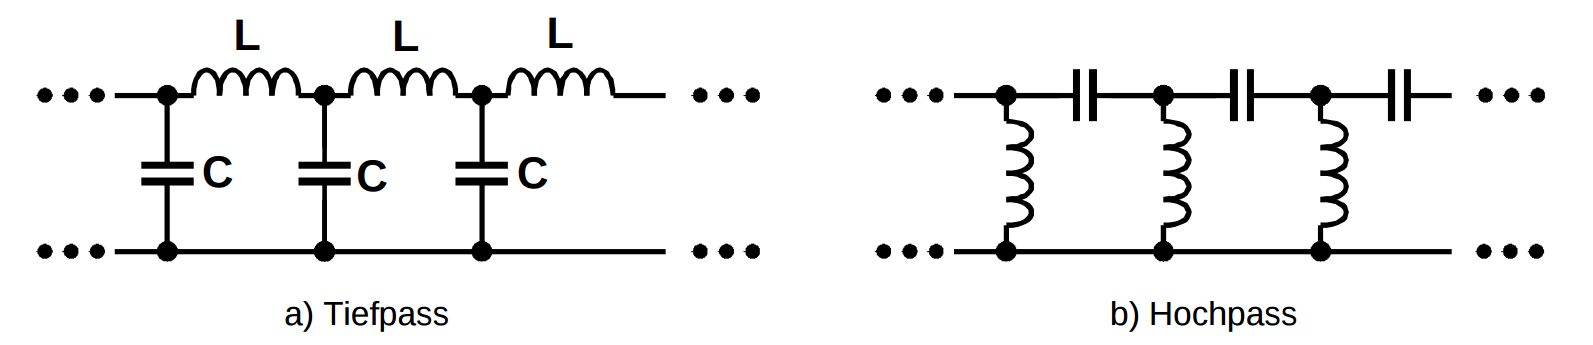
\includegraphics[width=0.8\textwidth]{V3561.png}
  \caption{Schematischer Aufbau von einem Hochpass und einem Tiefpass \cite{anleitung}.}
  \label{fig:V3561}
\end{figure}
In diesem Versuch sind alle LC-Glieder als Tiefpass aufgebaut. Sie filtern also
alle hohen Frequenzen eines Signals heraus. Es wird zunächst ein Tiefpass in
einer als unendlich lang simulierten LC-Kette betrachtet. Für diese Kette gilt
mit Hilfe der Kirchhoffschen Regeln:
\begin{equation}
  \omega²\,=\,\frac{2}{LC}\cdot(1-\cos(\theta)).
  \label{eqn:dispersionsrelationLC}
\end{equation}
$\omega$ kann dabei nur folgende Werte annehmen:
\begin{equation}
  0\,\le\,\omega\,<\,\frac{2}{\sqrt{LC}}.
  \label{eqn:grenzwertdispersLC}
\end{equation}
Das ist der Fall, da die LC-Kette, analog zu einem Tiefpass, Frequenzen ab einer
bestimmten Frequenz rausfiltert.
Diese Gleichung wird als Dispersionsrelation bezeichnet. Diese stellt die
Phasenänderung pro Kettenglied in Abhängigkeit von der Kreisfrequenz dar.
In Abbildung \ref{fig:V3562} zu sehen ist der Aufbau einer $LC_1C_2$-Kette.
Hier sind zwei unterschiedliche Kondensatoren in der Schaltung verbaut.
\begin{figure}[htb]
  \centering
  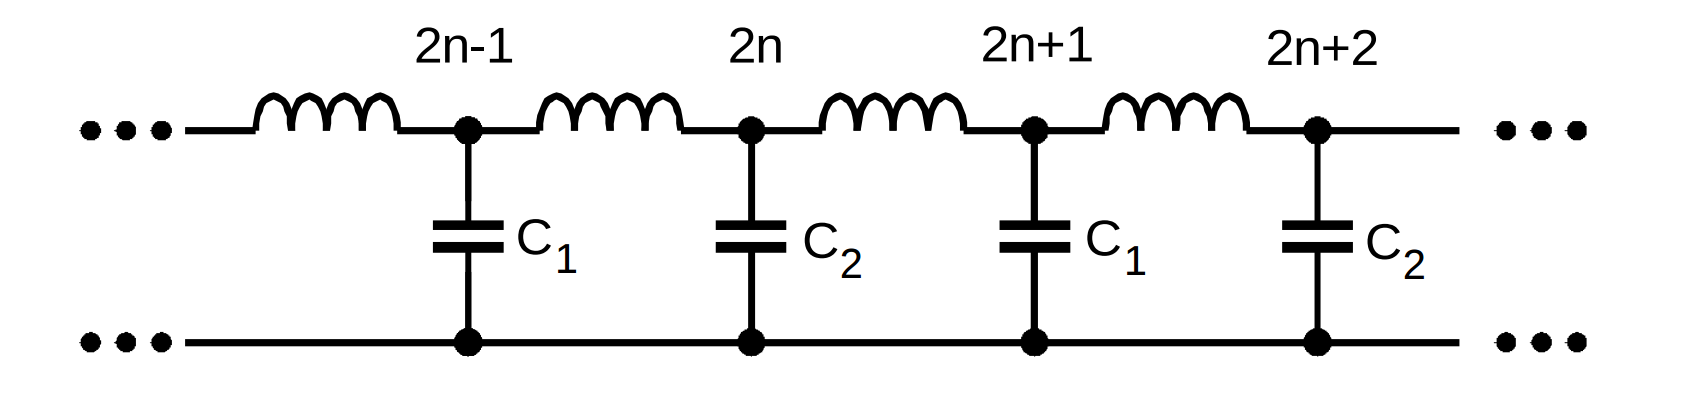
\includegraphics[width=0.8\textwidth]{V3562.png}
  \caption{Aufbau einer LC-Kette mit alternierenden Kettengliedern \cite{anleitung}.}
  \label{fig:V3562}
\end{figure}
Die Formel der durchgelassenen Frequenzen ist von der Kapazität abhängig und muss
daher nun abgeändert werden, damit ergibt sich dann:
\begin{equation}
  (\omega_{1/2})^2\,=\,\frac{1}{L}\left(\frac{1}{C_1}+\frac{1}{C_2}\right)\,\pm\,\frac{1}{L}\sqrt{\left(\frac{1}{C_1}+\frac{1}{C_2}\right)^2-\frac{4\sin^2(\theta)}{C_1C_2}}.
  \label{eqn:husoformel}
\end{equation}
$\omega$ hat dabei die drei Grenzwerte $\sqrt{\frac{2}{LC_1}}$,
$\sqrt{\frac{2}{LC_2}}$ und $\sqrt{\frac{2}{L}\frac{C_1+C_2}{C_1C_2}}$, die
dann zu dem in Abbildung \ref{fig:V3564} dargestelltem Graphen führen. Von dem
Graphen wird die Dispersionskurve für eine alternierende LC-Kette dargestellt.
Im Ursprung beginnt die Dispersionskurve und erreicht ihr Maximum
$\omega_2=\sqrt{\frac{2}{LC_1}}$ an der Stelle $\theta=\frac{\pi}{2}$.
Für $\theta=\frac{\pi}{2}$ wird der Minimalwert der Kreisfrequenz erzeugt,
also $\omega_1=\sqrt{\frac{2}{LC_2}}$.
Für $\theta=0$ bekommt man den Wert $\omega_1(0)=\sqrt{\frac{2}{L}\frac{C_1+C_2}{C_1C_2}}$.
\begin{figure}[htb]
  \centering
  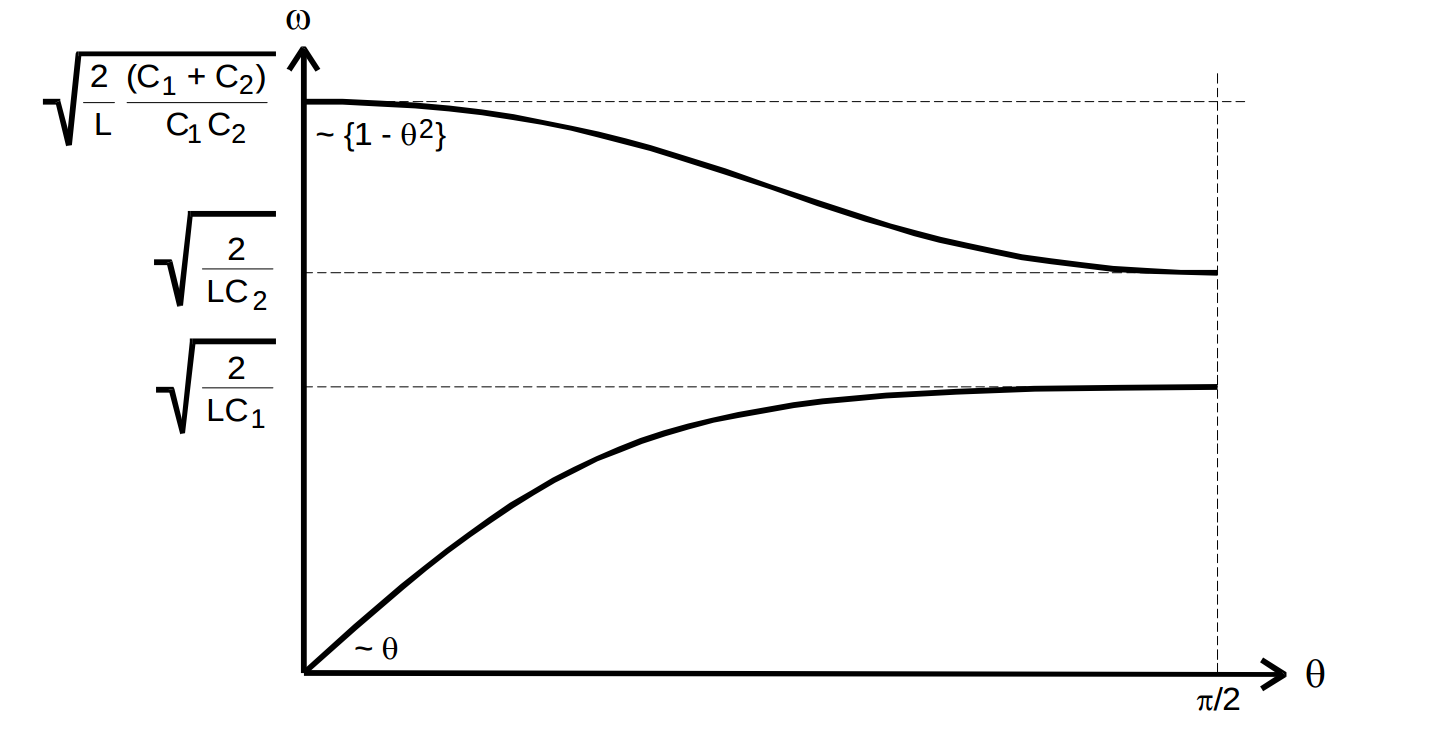
\includegraphics[width=0.8\textwidth]{V3564.png}
  \caption{Dispersionskurve einer alternierenden LC-Kette \cite{anleitung}.}
  \label{fig:V3564}
\end{figure}
Der Graph besteht aus zwei Kurven. Die obere Kurve ist die optische Kurve, da
diese Frequenzen hoch sind und die untere Kurve heißt akustische Kurve, da diese
Frequenzen tief sind. Der Grund dafür, dass zwei Kurven existieren ist das
wechselnde Vorzeichen in \eqref{eqn:husoformel}. Die durchgelassenen Frequenzen
sind daher endlich.\\
\\
Trivialerweise ist Abbildung \ref{fig:V3562} schwingfähig. Daher besitzt dieses System
Eigenfrequenzen und kann somit ohne äußere Einflüsse schwingen. Diese
Eigenfrequenzen können bestimmt werden, da nun die Enden der LC-Ketten offen
sind, also mit getrenntem Abschlusswiderstand $\left( Z \to \infty \right)$.
Es werden also die Spannungswellen ohne Phasensprung an den Enden reflekiert.
Es ist auch möglich, durch minimieren des Abschlusswiderstandes $\left( Z \to 0 \right)$
eine stehende Welle zu erzeugen, in dem Fall mit festen Enden. Dies wird in dem
Versuch allerdings nicht betrachtet.
Das Spektrum der Frequenzen hängt von vielen Gerätspezifischen Beschaffenheiten
ab. Zum Beispiel von der Dispersionsrelation, die für eine frequenzabhängige
Phasengeschwindigkeit und damit eine frequenzabhängige Wellenlänge sorgt, die
für stehende Wellen auf die Kette passen muss. Die entstehenden Eigenfrequenzen
sind messbar am Kettenende in Form eines Maximums der Spannungsamplitude. Damit
folgt für den Zusammenhang der verschiedenen Phasen:
\begin{equation}
  n_{max}\cdot\theta_k=k\cdot\pi
\end{equation}
k ist dabei definiert für
\begin{equation}
  k=1,2,3,...,n_{max}
\end{equation}
Bei $n_{max}$ wird die Phase betrachtet, die am Kettenende vorliegt. In
Abbildung \ref{fig:V3567} zu sehen ist, wie die nun entstandene stehende
Welle aussieht. Die einlaufende und die reflektierte Welle überlagern sich so,
dass die Phasenverschiebungen 0 oder ein vielfaches von $\pi$ sind. Das widerum
liegt daran, dass es an dem offenen Ende nicht zu einem Phasensprung kommt.
\begin{figure}[htb]
  \centering
  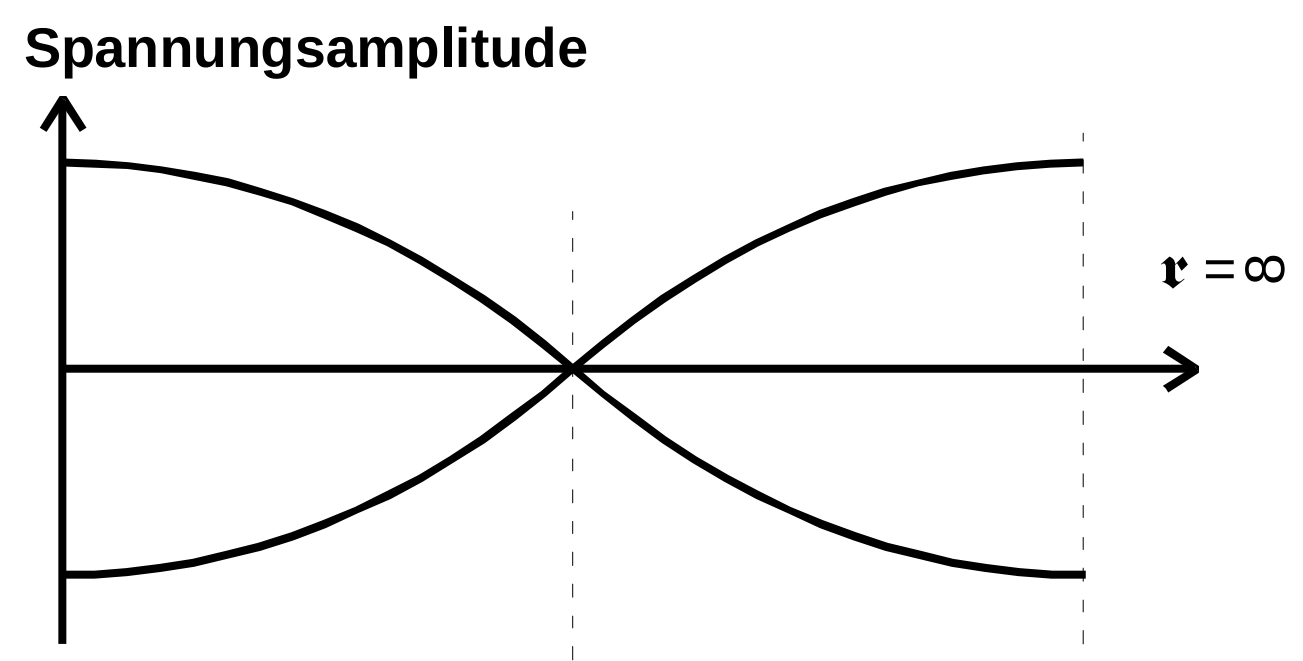
\includegraphics[width=0.5\textwidth]{V3567.png}
  \caption{Spannungsamplitude einer stehenden Welle \cite{anleitung}.}
  \label{fig:V3567}
\end{figure}
Die Anzahl der Kettenglieder bestimmt die Anzahl an möglichen stehenden Wellen.
Wenn am Kettenende kein Widerstand vorliegt kann sich allerdings auch eine
stehende Welle ausbilden. Auch hier muss dann die stehende Welle mit ihrer
Wellenlänge auf die Wellenlänge der Kette passen. \\
\\
Die Phasengeschwindigkeit ist die Ausbreitungsgeschwindigkeit von einer Welle
in der Kettenschaltung. Solange die einzelnen Frequenzkomponenten einer Welle
sich mit einer einheitlichen Phasengeschwindigkeit fortpflanzen, wird sich auch
die jeweilige Wellengruppe mit der Phasengeschwindigkeit ausbreiten.
Mit Hilfe der Dispersionsrelation ergibt sich dann für die Phasengeschwindigkeit:
\begin{equation}
  v_{Ph}\,=\,\frac{\omega}{\theta}\,=\,\frac{\omega}{\arccos(1-\frac{1}{2}\omega^2LC)}.
  \label{eqn:phasengesch}
\end{equation}

\section{Durchführung}
\label{durchführung}
Als erstes wurde die Durchlasskurve zweier LC-Ketten gemessen. Die dafür
genutzte Schaltung ist in Abbildung \ref{fig:V3568} zu sehen.
\begin{figure}[htb]
  \centering
  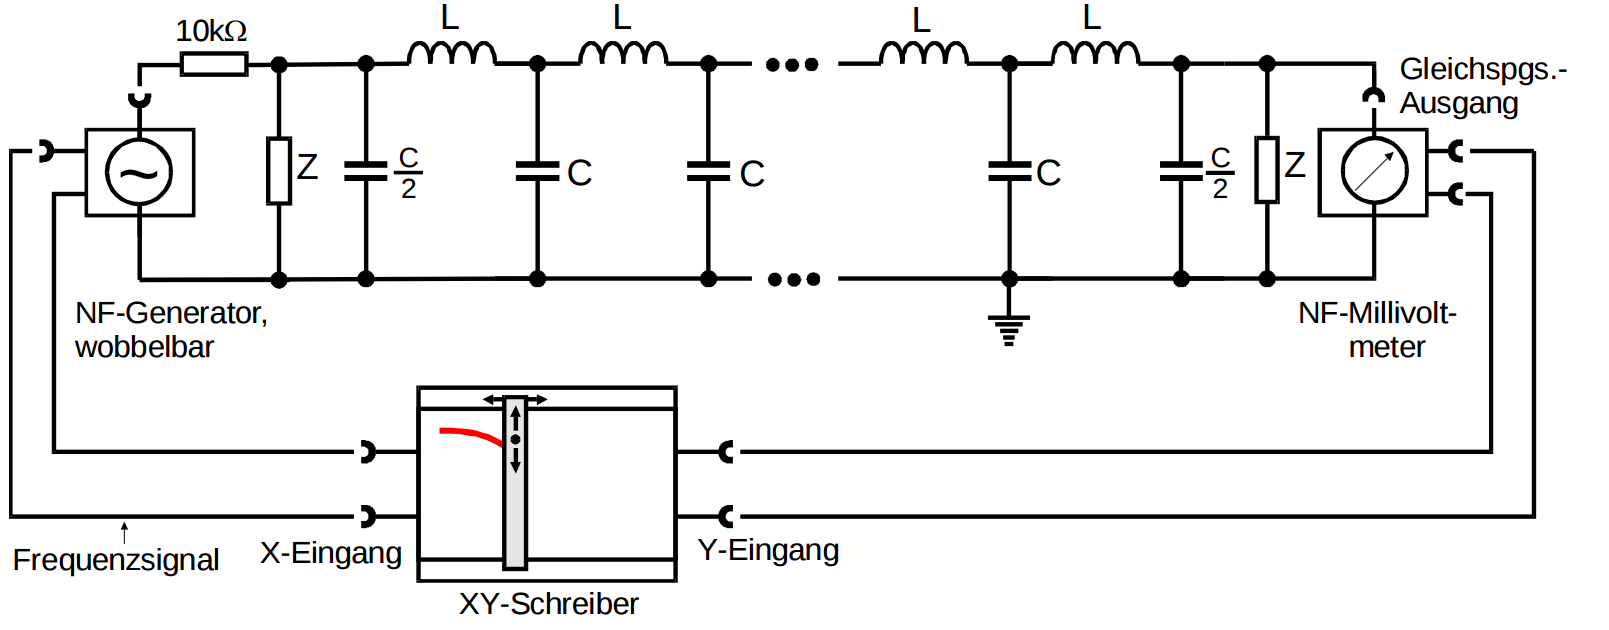
\includegraphics[width=0.8\textwidth]{V3568.png}
  \caption{Versuchsaufbau zur Messung der Durchlasskurve \cite{anleitung}.}
  \label{fig:V3568}
\end{figure}
Die Kette bestand aus 16 Kettengliedern.
Die Parameter der Induktivität $L$, der Kapazität $C_1$ und Kapazität
$C_2$ waren mit der Apparatur gegeben mit:
\begin{align}
  L &= \SI{1.75}{\milli\henry} \\
  C_1 &= \SI{22}{\nano\farad} \\
  C_2 &= \SI{9.39}{\nano\farad}.
\end{align}
Zuerst wurde der Wellenwiderstand sowohl für die $LC_1$ als auch für die
$LC_1C_2$-Kette gemessen. Die Werte der Wellenwiderstände ergeben sich mit den
Formeln:
\begin{align}
  &Z =\sqrt{\frac{L}{C}}=\SI{282}{\ohm}&(LC-Kette)& \\
  &Z =\sqrt{\frac{2L}{C_1+C_2}}=\SI{334}{\ohm}&\mathup{(LC_1C_2-Kette)}&. \\
\end{align}

Die Durchlasskurve, also die Ausgangsamplitude in Abhängigkeit von der Frequenz,
wurde daraufhin mit einem XY-Schreiber aufgenommen. Auf
dieser wurde dann an 5 verschiedenen Stellen die Frequenz der Eingansspannung
notiert, um damit eine Skala für die Aufzeichnung zu erhalten.
Bei der $LC_1C_2$-Kette mit alternierenden Kapazitäten wird die Kapazität jedes
zweiten Kondensators verändert und dann erneut die gleiche Messung durchgeführt.\\
\\
Als nächstes wird die Dispersionsrelation gemessen. Die dafür genutzte Schaltung
ist in Abbildung \ref{fig:V3569} zu sehen.

\begin{figure}
  \centering
  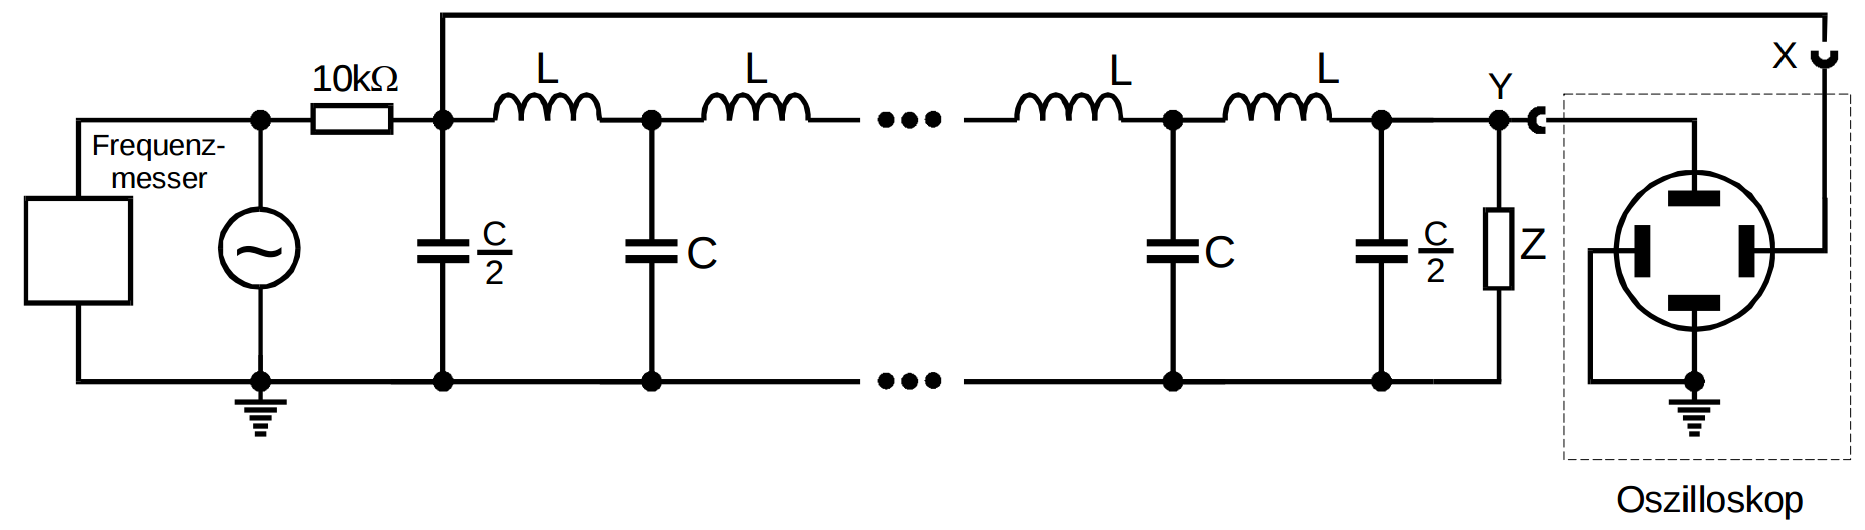
\includegraphics[width=0.8\textwidth]{V3569.png}
  \caption{Versuchsaufbau zur Aufnahme der Dispersionsrelation \cite{anleitung}.}
  \label{fig:V3569}
\end{figure}
Auf dem Oszilloskop sind dabei Lissajous-Figuren zu beobachten. An den Figuren
ist die jeweilige Phasenverschiebung zu sehen. Für beide Ketten wird immer, wenn
die Phasenverschiebung ein vielfaches von $\pi$ beträgt, die entsprechende
Frequenz notiert, bis keine Figur mehr zu erkennen ist.\\
\\
Als letztes wird die Spannungsamplitude der $LC$-Kette an dem jeweiligen
Kettenglied gemessen. Dazu werden die Eigenfrequenzen der ersten beiden Moden
eingestellt. Diese liegen bei \SI{5}{\kilo\hertz} und \SI{10}{\kilo\hertz} vor.
Gemessen wird für beide Frequenzen mit offenen Enden
(Abschlusswiderstand getrennt) und für eine Frequenz mit aktivierten
Abschlusswiderständen.
\clearpage
\section{Auswertung}
\label{sec:auswertung}
\subsection{Bestimmung der Grenzfrequenzen}
An den Markierungen auf den Zeichnungen des XY-Schreibers wurden die in Tabelle \ref{tab:messwerte1}
stehenden Werte für die Frequenz gemessen.
\begin{table}
  \centering
  \caption{Werte der Freqenz an den verschiedenen Punkten der Skala.}
  \label{tab:messwerte1}
  \sisetup{table-format=5.0}
  \begin{tabular}{S[table-format=2.0] S S[table-format=2.0] S}
    \toprule
    \multicolumn{2}{c}{$LC - \text{Kette}$} & \multicolumn{2}{c}{$LC_1C_2 - \text{Kette}$}\\
    {Abstand in $\si{cm}$} & {$f \,/\, \si{\hertz}$} & {Abstand in $\si{cm}$} & {$f \,/\, \si{\hertz}$}\\
    \midrule
    3 & 31713 & 3 & 32822\\
    6 & 36077 & 6 & 39054\\
    9 & 41028 & 9 & 46170\\
    12 & 46567 & 12 & 53910\\
    16 & 54687 & 15 & 62620\\
    \bottomrule
  \end{tabular}
\end{table}\\
Zur Bestimmung der Grenzfrequenzen wird zunächst ein Referenzpunkt auf dem Papier gewählt.
Mittels Python wird dann der Abstand auf dem Papier als Funktion der Frequenz nach
\begin{equation}
  x \left( f \right) = a \cdot \log \left( \left| f \right| \right) + b
  \label{eqn:fit1}
\end{equation}
gefittet. Durch Umkehren der Funktion und Einsetzen des geometrisch bestimmten Abstands
ergeben sich die jeweiligen Grenzfrequenzen.
Die Funktion $f \left( x \right)$ lautet dann
\begin{equation}
  f \left( x \right) =  e^{\frac{x-b}{a}}
  \label{eqn:fit2}
\end{equation}
mit den Parametern
\begin{equation}
  a= \SI{23.8(2)}{\centi\meter}
\end{equation}
und
\begin{equation}
  b= \SI{-244(2)}{\centi\meter}
\end{equation}
für die $LC$-Kette bzw.
\begin{equation}
  a= \SI{18.6(3)}{\centi\meter}
\end{equation}
und
\begin{equation}
  b= \SI{-190(4)}{\centi\meter}
\end{equation}
für die $LC_1C_2$-Kette.
\\
Die Grenzfrequenz, der $LC$-Kette, liegt bei $\SI{14.2}{\centi\meter}$ auf dem Papier
und damit bei
\begin{equation}
  f = \SI{50.899}{\kilo\hertz}.
\end{equation}
Nach \eqref{eqn:grenzwertdispersLC} ist mit den gegebenen Induktivitäten und Kapazitäten der Literaturwert
dafür
\begin{equation}
  f = \SI{51.3}{\kilo\hertz}
\end{equation}
und die relative Abweichung des gemessenen Wertes
beträgt $\SI{0.8}{\percent}$.
\clearpage
Die Grenze, des akustischen Astes, der $LC_1C_2$-Kette, befindet sich bei $\SI{4.5}{\centi\meter}$ auf dem Papier.
Das entspricht einer Fregenz von
\begin{equation}
  f = \SI{35.879}{\kilo\hertz}.
\end{equation}
Der optische Ast beginnt bei $\SI{12.5}{\centi\meter}$ und endet bei $\SI{15.9}{\centi\meter}$.
Die Frequenzen dazu liegen dann bei
\begin{equation}
  f = \SI{55.207}{\kilo\hertz}
\end{equation}
bis
\begin{equation}
  f = \SI{66.303}{\kilo\hertz}.
\end{equation}
Zu den starken Schwankungen kommt es, da zuvor der Abschlusswiderstand auf den Wellenwiderstand
bei $\omega = 0$ eingestellt wurde. Da der Wellenwiderstand von $\omega$ abhängt
passt der zuvor eingestellte Wert, wenn die Frequenz erhöht wird, nicht mehr zur
Welle. Es kommt zu Reflexionen. Bei bestimmten Frequenzen können sich stehende Wellen
ausbilden, was sich dann in den Aufzeichnungen in Form dieser Schwankungen zeigt.
Nach den Grenzwerten von Formel \eqref{eqn:husoformel} folgen die Literaturwerte
und relativen Abweichungen:
\begin{align}
  &f = \SI{36.275}{\kilo\hertz} & &\SI{1.1}{\percent} & &\text{(Grenze akustischer Ast)}\\
  &f = \SI{55.524}{\kilo\hertz} & &\SI{0.6}{\percent} & &\text{(Anfang optischer Ast)}\\
  &f = \SI{66.324}{\kilo\hertz} & &\SI{0.03}{\percent} & &\text{(Ende optischer Ast)}
\end{align}

\subsection{Dispersionskurven}
\begin{table}
  \centering
  \caption{Werte der Freqenz zur entsprechenden gesamten Phasenverschiebung $n \cdot \pi$.}
  \label{tab:messwerte2}
  \sisetup{table-format=5.0}
  \begin{tabular}{S[table-format=1.0] S S}
    \toprule
    & {$LC - \text{Kette}$} & {$LC_1C_2 - \text{Kette}$}\\
    {$n$} & {$f \,/\, \si{\hertz}$} & {$f \,/\, \si{\hertz}$}\\
    \midrule
    1 & 5015 & 5725\\
    2 & 9950 & 11550\\
    3 & 14900 & 17125\\
    4 & 19580 & 22380\\
    5 & 24220 & 27210\\
    6 & 28550 & 31490\\
    7 & 32400 & 34830\\
    8 & 36100 & 38710\\
    9 & 39550 & \\
    10 & 42300 & \\
    11 & 45200 & \\
    12 & 47150 & \\
    13 & 48900 & \\
    14 & 50140 & \\
    \bottomrule
  \end{tabular}
\end{table}
In Tabelle \ref{tab:messwerte2} stehen die Frequenzen zu den mit den Lissajous-Figuren
bestimmten Phasenverschiebungen. Dabei steht $n$ für das $n$-Fache von $\pi$.
Außerdem liegt bei $n = 1$ die Grundschwingung und bei jedem weiteren $n$ die $n-1$-te
oberschwingung vor.\\
Nun wird nach Formel \eqref{eqn:dispersionsrelationLC} die Dispersionskurve der $LC$-Kette berechnet und
zusammen mit den gemessenen Werten aus Tabelle \ref{tab:messwerte2} in den Graphen
\ref{fig:plot} eingetragen.
\begin{figure}
  \centering
  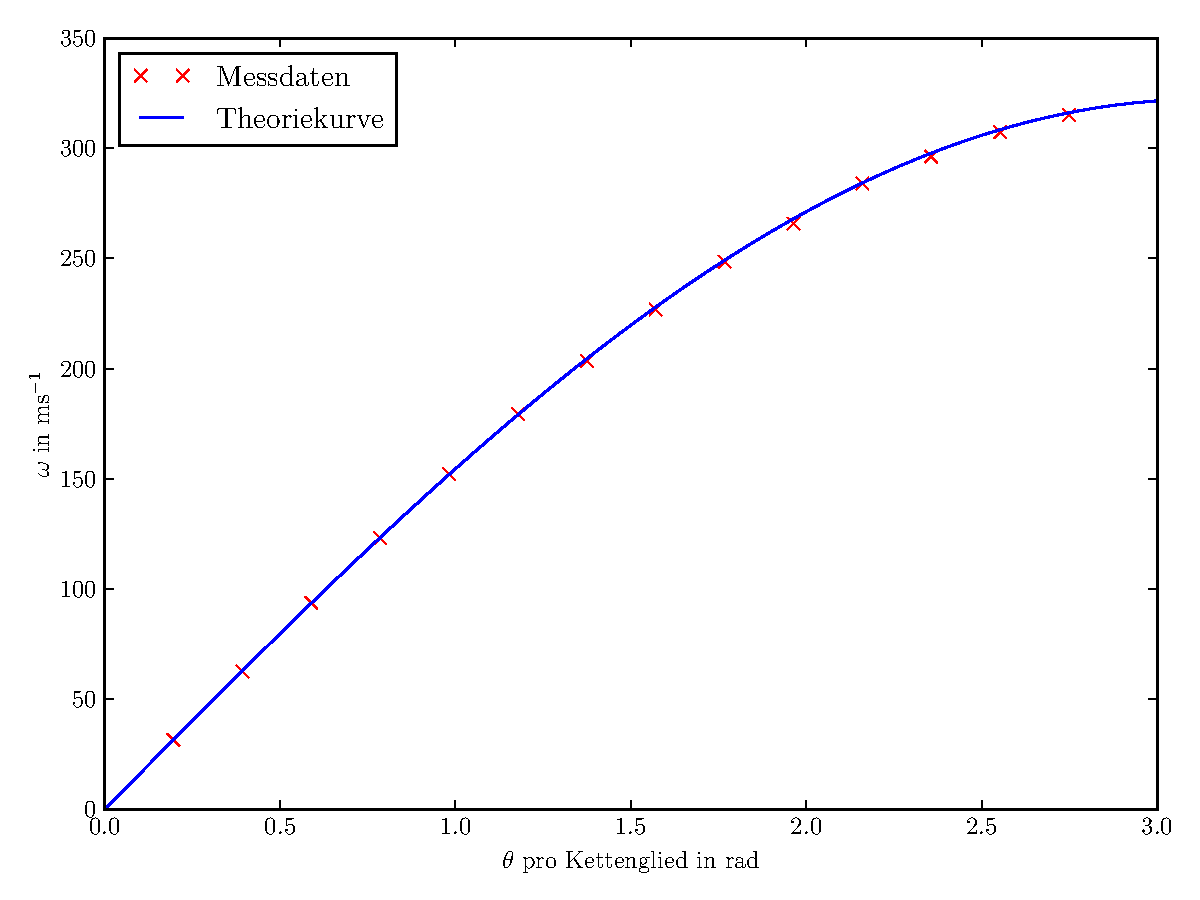
\includegraphics[width=\textwidth]{Plot3.pdf}
  \caption{Dispersionskurve $LC$-Kette.}
  \label{fig:plot}
\end{figure}\\
An dem Graphen ist zu sehen, dass sich die Kreisfrequenz bei einem Phasenwinkel
von $\pi$ einer Grenze von etwa $320\,\si{\milli\second\tothe{-1}}$ nähert. Das entspricht
also einer Frequenz von etwa $\SI{51}{\kilo\hertz}$.
\clearpage
Nach Formel \eqref{eqn:husoformel} ergibt sich, mit dem negativen Vorzeichen vor der Wurzel, der
akustische Ast der $LC_1C_2$-Kette während das positive Vorzeichen vor der Wurzel
zu dem optischen Ast führt.
Beide Varianten, der Funktion, sind in Abbildung \ref{fig:plot2}, zusammen mit den gemessenen
Werten, aufgetragen.
\begin{figure}
  \centering
  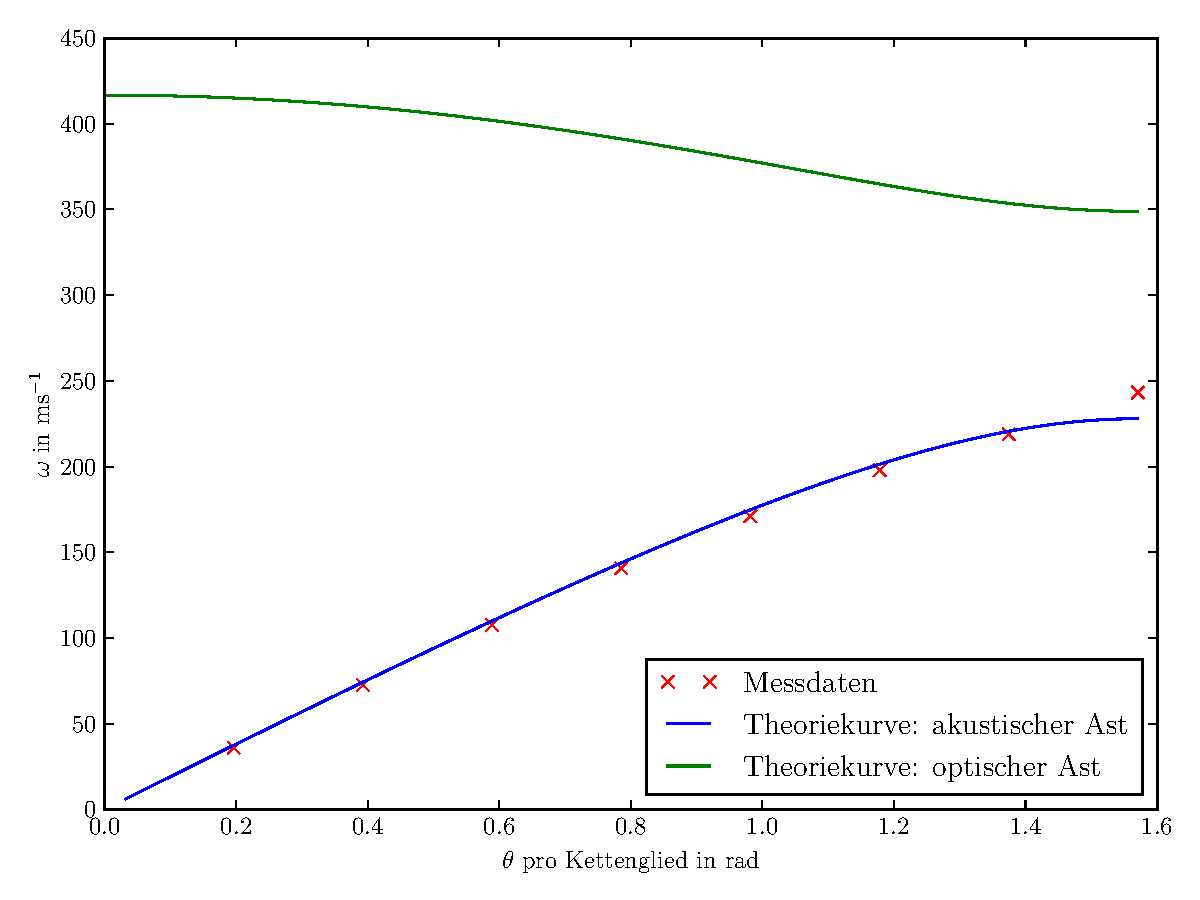
\includegraphics[width=\textwidth]{Plot4.pdf}
  \caption{Dispersionskurve $LC_1C_2$-Kette.}
  \label{fig:plot2}
\end{figure}\\
Zu erkennen ist, dass sich der akustische Ast einer Kreisfrequenz von ca. $230\,\si{\milli\second\tothe{-1}}$
bzw. einer Frequenz von $\SI{36}{\kilo\hertz}$ nähert.
Außerdem befindet sich zwischen den Kreisfrequenzen $350\,\si{\milli\second\tothe{-1}} \left( \SI{56}{\kilo\hertz} \right)$
und $420\,\si{\milli\second\tothe{-1}} \left( \SI{67}{\kilo\hertz} \right)$ die Theoriekurve
des optischen Astes.
\clearpage
\subsection{Berechnung der Phasengeschindigkeit}
Um die Phasengeschwindigkeit der verschiedenen Eigenmoden zu bestimmen, wird der Quotient
aus der Kreisfrequenz und der Phase berechnet. Die Ergebnisse davon stehen in Tabelle
\ref{tab:phasengeschwindigkeiten}. Diese werden zusammen mit der Theoriekurve nach
Formel \eqref{eqn:phasengesch}, wie in Abbildung \ref{fig:plot3} aufgetragen.
\begin{table}
  \centering
  \caption{Phasengeschwindigkeiten, der Wellen bei entsprechender Kreisfrequenz ($LC$-Kette).}
  \label{tab:phasengeschwindigkeiten}
  \sisetup{table-format=5.0}
  \begin{tabular}{S S[table-format=6.0]}
    \toprule
    {$f \,/\, \si{\hertz}$} & {$v_\mathup{Ph} \,/\, \si{\second\tothe{-1}}$}\\
    \midrule
    5015 & 160480\\
    9950 & 159200\\
    14900 & 158933\\
    19580 & 156640\\
    24220 & 155008\\
    28550 & 152267\\
    32400 & 148114\\
    36100 & 144400\\
    39550 & 140622\\
    42300 & 135360\\
    45200 & 131491\\
    47150 & 125733\\
    48900 & 120369\\
    50140 & 114606\\
    \bottomrule
  \end{tabular}
\end{table}
\begin{figure}
  \centering
  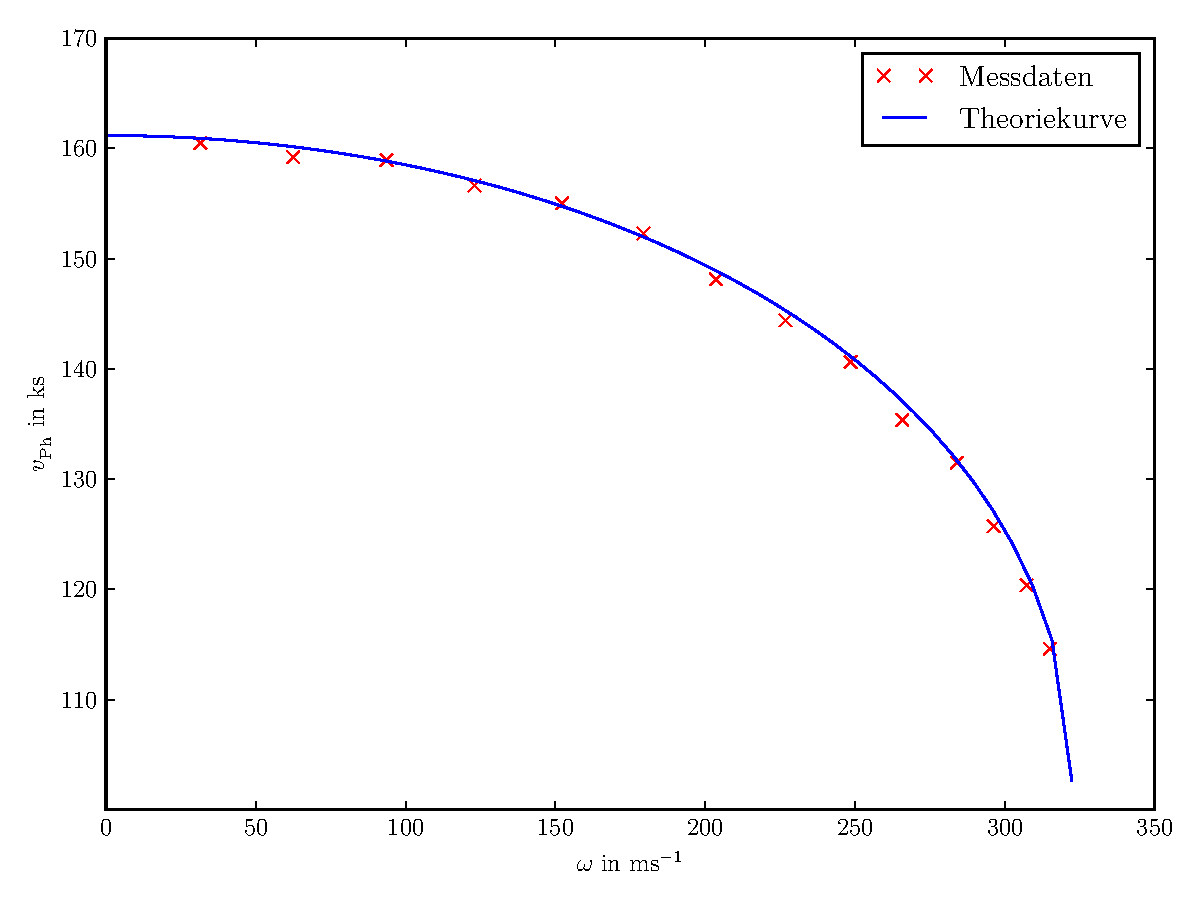
\includegraphics[width=\textwidth]{Plot6.pdf}
  \caption{Phasengeschwindigkeit in Abhängigkeit von der Kreisfrequenz.}
  \label{fig:plot3}
\end{figure}\\
In dem Graphen ist zu sehen, dass die Phasengeschwindigkeit bei zunehmender Frequenz immer stärker
abnimmt und die Kreisfrequenz dabei gegen die Grenzfrequenz läuft.
\clearpage
\subsection{Messung des Verlaufs der Stehenden Wellen bei $\SI{5}{\kilo\hertz}$ und $\SI{10}{\kilo\hertz}$}
In Tabelle \ref{tab:messwerte3} stehen die gemessenen Spannungen am $n$-ten Kettenglied
bei einer Frequenz von $\SI{5}{\kilo\hertz}$ bzw. $\SI{10}{\kilo\hertz}$ (also Grundschwingung und erste Oberschwingung).
\begin{table}
  \centering
  \caption{Spannung am $n$-ten Kettenglied.}
  \label{tab:messwerte3}
  \sisetup{table-format=2.2}
  \begin{tabular}{S[table-format=1.0] S S S[table-format=1.3]}
    \toprule
    & {$f = \SI{5}{\kilo\hertz}$} & {$f = \SI{10}{\kilo\hertz}$} & {$f = \SI{5}{\kilo\hertz}$}\\
    {$n$} & \multicolumn{3}{c}{$U \,/\, \si{\volt}$}\\
    \midrule
    0 & 17.25 & 16.5 & 0.325\\
    1 & 16.25 & 14.5 & 0.325\\
    2 & 15 & 11 & 0.320\\
    3 & 13 & 6 & 0.315\\
    4 & 11 & 0.25 & 0.310\\
    5 & 8.5 & 6 & 0.315\\
    6 & 6 & 11.5 & 0.320\\
    7 & 3 & 15.5 & 0.325\\
    8 & 0.25 & 16.75 & 0.325\\
    9 & 2.75 & 16 & 0.320\\
    10 & 5.5 & 12.25 & 0.315\\
    11 & 8 & 6.5 & 0.310\\
    12 & 10 & 0.25 & 0.310\\
    13 & 11.75 & 6.5 & 0.315\\
    14 & 13.25 & 11.25 & 0.320\\
    15 & 13.75 & 16 & 0.325\\
    16 & 14.5 & 17.5 & 0.325\\
    \bottomrule
  \end{tabular}
\end{table}\\
Nun wird die an den einzelnen Kettengliedern gemessene Spannung gegen die Nummer
des jeweiligen Kettengliedes aufgetragen. Die Punkte wurden dabei miteinander verbunden
um eine deutlichere und übersichtlichere Gestalt der Kurven zu erhalten.\\
\clearpage
\begin{figure}
  \centering
  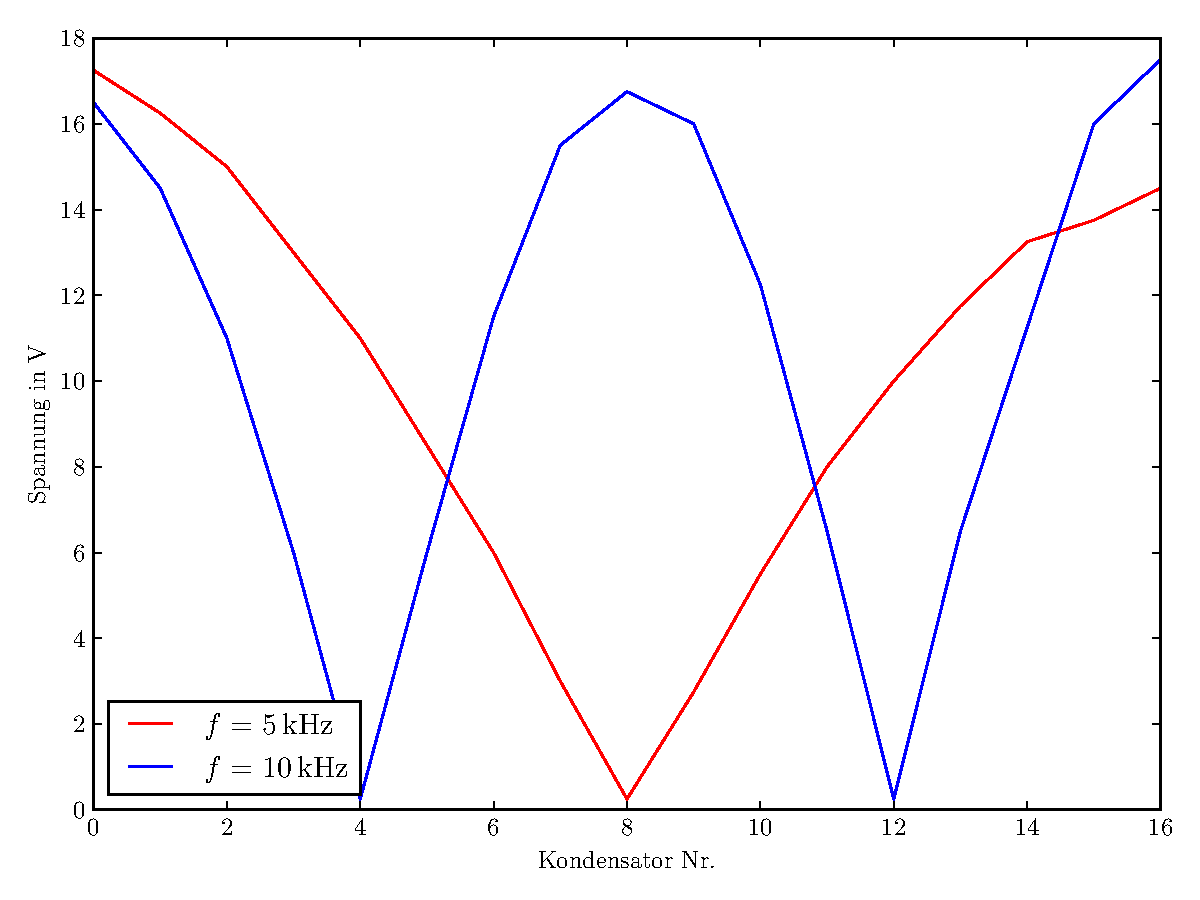
\includegraphics[width=\textwidth]{Plot5.pdf}
  \caption{Spannung an den einzelnen Kettengliedern.}
  \label{fig:plot4}
\end{figure}
Zu sehen sind die Maxima an den Rändern, sowie ein (Grundschwingung) bzw. zwei (erste Oberschwingung)
Knoten dazwischen.
\clearpage
\begin{figure}
  \centering
  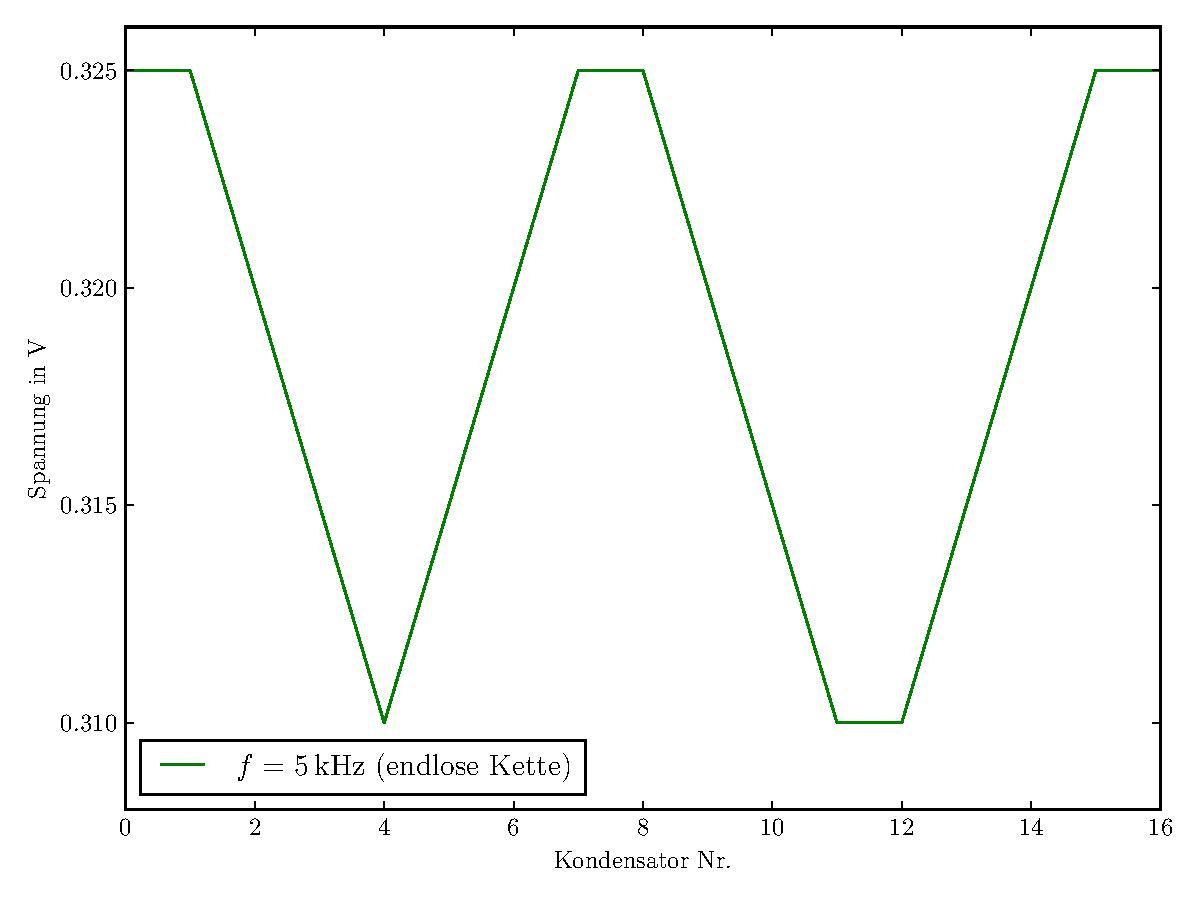
\includegraphics[width=\textwidth]{Plot7.pdf}
  \caption{Spannung an den einzelnen Kettengliedern (endlose Kette).}
  \label{fig:plot5}
\end{figure}
Die grüne Kurve in Abbildung \ref{fig:plot5} soll zeigen, dass die Spannung bei
einer endlosen Kette annähernd konstant ist.
\clearpage
\section{Diskussion}
\label{sec:diskussion}
Insgesamt fällt auf, dass der Versuch sehr gute Werte liefert. Die Abweichungen
sind verschwindend gering. Der Unterschied zwischen den gemessenen Grenzfrequenzen
\begin{align}
  &LC\text{-Kette:} & &\SI{50.899}{\kilo\hertz}\\
  &LC_1C_2\text{-Kette:} & &\SI{35.879}{\kilo\hertz}\\
  & & &\SI{55.207}{\kilo\hertz}\\
  & & &\SI{66.303}{\kilo\hertz}
\end{align}
und den rechnerisch bestimmten Werten liegt im Bereich von $\SI{0.03}{\percent}$
bis $\SI{1.1}{\percent}$.\\

Die Dispersionskurve und die Kurve der Phasengeschwindigkeit der $LC$-Kette sind
sehr genau. Bei der $LC_1C_2$-Kette weicht der letzte gemessene Wert etwas weiter
ab. Eine Fehlerquelle ist, dass der Generator seine Frequenz ständig abändert, was
dazu führt, dass sich beim bestimmen der Frequenzen mit den Lissajous-Figuren
Abweichungen einschleichen können. Leichte Schwankungen der Werte z.B. bei dem
Spannungsverlauf der endlosen Kette könnten dadurch zustande kommen, dass die
Widerstände an den Enden nicht exakt auf den Wellenwiderstand eingestellt sind,
wodurch es zu schwachen Reflexionen kommen kann.
\clearpage
\nocite{*}
\printbibliography

\end{document}
